\section{Flexible resource allocation mechanisms}
\label{sec:flexible-resource-allocation-mechanisms}
As explained earlier, previous research outlined in Section~\ref{sec:introduction} does not consider resource-elastic tasks. Therefore, in this section, we propose three mechanisms for solving our optimisation problem: an approximation algorithm and two auction-based mechanisms. As the greedy algorithm is a centralised approximation algorithm it has several shortcomings: it assumes that users reveal private task information truthfully, and it assumes there is a central point of control for all server allocation decisions. We address each of these shortcomings in the subsequent two auction mechanisms. 

\subsection{Greedy algorithm}
\label{subsec:greedy-algorithm}
To solve knapsack problems, a greedy approximation algorithm is often used~\cite{sahni1975approximate}. Therefore, we have applied a similar approach to our problem. However, due to the elastic nature of task resources, a novel additional stage is required. More specifically, the greedy algorithm (pseudo code can be found in Section 2 of the supplementary material) has two stages: the first stage sorts the tasks based on a task priority function. The novel second stage uses the sorted tasks to apply two heuristics; the first for selecting a server based on available server resources and the second to allocate resources based on the available server resources and the required resources of the task. %% TODO Add an explanation about the heuristics

\subsubsection{Lower bound of the greedy algorithm}
\label{subsubsec:greedy-lower-bound}
%% TODO look at again
Due to the server selection and resource allocation heuristics not taking into account other tasks, the lower bound of the greedy algorithm is $\frac{1}{OPT}$ (where $OPT$ is the optimal social welfare) where the task value is used for the task priority function. However in testing, we found that the task value is not the best task priority heuristic as it does not consider the effect of deadlines or the required resources of the task. This is due to not considering other tasks resource requirements when allocating resources, no matter of the server selection or resource allocation functions, the algorithm cannot guarantee that any subsequent tasks could be allocated to any server after the first task is allocated. As a result, the algorithm can be guaranteed to achieve at least $\frac{1}{OPT}$ of the optimal social welfare by sorting the tasks by task value ($v(j) = j_v$).

\subsubsection{Computational complexity of greedy algorithm}
\label{subsubsec:greedy-time-complexity}
The computational complexity of the greedy algorithm is $O(\left|J\right| \left|I\right| + n^3)$, where $\left|J\right|$ is the number of tasks, $\left|I\right|$ is the number of servers and $n$ is the discretization of the server and task resources. This assumes that all of the heuristics take constant complexity for their evaluation. Therefore, for the first stage of the algorithm where the tasks are sorted the complexity is $O(\left|J\right| \log(\left|J\right|))$. While for the second stage, for each task the server selection heuristic is applied to each server, which has a complexity of $O(\left|J\right| \left|I\right|)$. Then for resource allocation, to get the best allocation requires checking if all of the server resources depends on the server discretization.\footnote{Faster solutions exist for finding the best allocations like branch and bound or Karush–Kuhn–Tucker conditions.} Therefore, the overall complexity is $O(\left|J\right| \log(\left|J\right|) + \left|J\right| \left|I\right| + n^3) = O(\left|J\right| \left|I\right| + n^3)$.

\subsection{Critical value auction}
\label{subsec:critical-value-auction}
A potential shortcoming of the greedy algorithm is that it assumes truthful reporting of the task characteristics, including its value. In realistic settings with self-interested task owners, if the greedy algorithm was used to allocate resources such that the value is the price paid, the system would be open to manipulation and the misreporting of task attributes. Therefore, in this section we propose the Critical Value auction, a strategyproof (weakly dominant incentive compatible) auction that means users have no incentive to misreport task attributes.

The auction is based on Single Parameter Auctions~\cite{nisan2007algorithmic} (Section~9.5.4), where the price for a task is the minimum value revealed by a task such that it would still be allocated to any server, called the \emph{critical value}. The auction (pseudo code can be found in Section 3 of the supplementary material) is implemented using the greedy algorithm, from Subsection~\ref{subsec:greedy-algorithm}, for finding both the initial allocation of tasks and critical value for each task (in a modified form). Because of this, the auction inherits the social welfare properties of the greedy algorithm using the same modular functions.

The auction works by first finding the initial allocation of tasks based on task's revealed values using the greedy algorithm. Then for each allocated task its critical value is determined that is equal to the minimum value the task could report such that it would still be allocated. This is done by modifying the greedy algorithm such that after every task is allocated to a server, a check is done to see if the critical value task could be allocated to any server.\footnote{This check has linear time complexity as it assumes that a server would allocate all of its available resources to the critical task. However, for the bandwidth resources, this must be split between loading and sending resources to check if the deadline can be met.} Once the critical value task cannot be allocated to any server, then the task priority of the previously allocated task must be equal to the critical value task's minimum task priority.\footnote{We assume that the critical task would be placed above the task if the task priorities are equal. To avoid this, the owner can add a small amount of the value to increase the task priority, placing the critical task ahead.} The critical value is found by taking the inverse of the task priority function with critical task's attributes and task priority of the previous task.

\subsubsection{Computational complexity of critical value auction}
\label{subsubsec:critical-value-auction-time-complexity}
Using the argument from Subsection~\ref{subsubsec:greedy-time-complexity}, the computational complexity of the greedy algorithm is $O(\left|J\right| \left|I\right|)$. The computational complexity of the auction is $O(\left|J\right|^2 \left|I\right|)$, as the auction repeats the greedy algorithm  $\left|J\right|$ times. For the first stage of the auction, the greedy algorithm finds the initial allocation, with the second stage finding the critical value of each allocated task. For the second stage, it uses a modified version of the greedy algorithm, which has a computational complexity of  $O(\left|J\right| \left|I\right|)$. After each task is allocated, a check runs to see if the critical task can be allocated to any server. This check has linear time complexity, as the server's bandwidth resources must be split between task loading and sending speeds. The second modification calculates a task's critical value that takes constant time. Therefore, the computational complexity is due to running  the greedy algorithm ($O(\left|J\right| \left|I\right|)$) plus the complexity of checking after each task for each server ($O(\left|J\right| \left|I\right|)$). Therefore the computational complexity for calculating the critical value of an individual task is $O(\left|J\right| \left|I\right|)$. Thus, combining the two, the overall time complexity is $O(\left|J\right|^2 \left|I\right|)$, as the critical value needs to be calculated for every task.

\subsubsection{Critical value auction strategyproof requirement}
\label{subsubsec:critical-value-auction-strategyproof}
Previous work~\cite{nisan2007algorithmic} (in particular Lemma~11.9) has proven that if the allocation decision is monotonic and critical value payments are used, then the auction is strategyproof (weakly dominant incentive compatible). In our setting, a monotonic allocation means that if an agent is allocated for a given set of parameters, say $\theta_j = (v_j, s_j, w_j, r_j, d_j)$, it would remain allocated when  reporting $\theta'_j = (v'_j, s'_j, w'_j, r'_j, d'_j) $, with $v'_j \geq v_j$, $s'_j \leq s_j$, $w'_j \leq w_j$, $r'_j \leq r_j$, and $d'_j \geq d_j$. This condition can be achieved by using a task priority function that enforces this monotonicity relationship. Specifically, reporting $\theta'_j$ must result in a task priority at least as high as reporting $\theta_j$. In this case, the agent would be evaluated earlier in the greedy order and if $\theta_j$ was allocated, $\theta'_j$ would also remain allocated. Here, it is important to enforce that agents are never allocated more than their requested $s_j$, $w_j$ and $r_j$, and that results are returned exactly on the deadline $d_j$, to ensure that truthful reporting of these parameters is incentivised (as agents maximise the task priority function in this way). This can be easily achieved by post-processing a given solution. One example family of task priority functions that meets the required monotonicity requirement is $\frac{\alpha(v_j, d_j)}{\beta(s_j, w_j, r_j)}$, where  $\alpha$ and $\beta$ are monotonically increasing in their parameters. In our experiments, we use $\frac{v_j \cdot d_j}{s_j + w_j + r_j}$.

\subsection{Decentralised iterative auction}
\label{subsec:decentralised-iterative-auction}
In some applications of edge computing, keeping the value of a task secret is important, especially if the infrastructure is shared by multiple companies or by partners of a military coalition. Therefore, we propose a novel decentralised iterative auction. In this auction, servers offer to complete tasks for a given price, which is equal to the sum of prices (i.e., the server's revenue) of other tasks that the task would displace, plus a bid increment. Task owners either reject or accept these prices, potentially displacing other tasks, and the process continues iteratively until the allocation converges.

%based on the pricing principle of the VCG auction~\cite{vickrey,Clarke,groves}. In the VCG auction, the price of an item is the difference in social welfare for when the item is sold and when it is not. Our proposed novel auction uses this VCG mechanism except using revenue instead of social welfare to calculate a price. This allows tasks to not need to reveal their task value to the servers as the task price (and not task value) is used to update task prices. 

\begin{algorithm}
    \caption{Decentralised iterative auction}
    \label{alg:decentralised-iterative-auction}
    \begin{algorithmic}
        \REQUIRE $J'$ is the set of unallocated tasks, initially the set of tasks
        \REQUIRE $I$ is the set of servers
        \REQUIRE $P(i, j)$ is the solution to the server revenue optimisation problem in Subsection~\ref{subsubsec:decentralised-iterative-problem} using the server $i$ and new task $j$. 
        \REQUIRE $\leftarrow_R A$ randomly select an element from set $A$
        
        \WHILE{$|J'| > 0$}
            \STATE{$j \leftarrow_R J'$}
            \STATE{$\min_p \leftarrow \infty$}
            \STATE{$\min_i \leftarrow \text{NULL}$}
            \FORALL{$i \in I$}
                \STATE{$p \leftarrow \max(R_i - P(i, j) + b_i, r_i)$}
                \IF{$p < \min_p$}
                    \STATE{$\min_p \leftarrow p$}
                    \STATE{$\min_i \leftarrow i$}
                \ENDIF
            \ENDFOR
            \IF{$\min_p \leq v_j$}
                \STATE{$p_j \leftarrow \min_p$}
                \STATE{$J_{\min_i} \leftarrow J_{\min_i} \cup \{j\}$}
                \STATE{Add deallocated tasks from server $\min_i$ to $J'$}
            \ENDIF
            \STATE{$J' \leftarrow J' \setminus \{j\}$}
        \ENDWHILE
    \end{algorithmic}
\end{algorithm}

Formally, tasks have a price, $p_j$, initially set to 0, while each server $i$ has four additional variables: $R_i$ for revenue, $b_i$ for bid increment, $r_i$ for reserve price and $J_i$ for the set of currently allocated task. 

The pseudo code for the auction is  shown in Algorithm~\ref{alg:decentralised-iterative-auction}. For simplicity, we show this as a sequential algorithm, but the respective owners of each task $j$ could be executing this in parallel and in a decentralised manner. In more detail, the auction  works by tasks individually advertising all of their attributes except their value to all of the servers, who each reply with a price to run. This price is the difference between the current server revenue and the revenue when the task is allocated with a price of zero (solved with the optimisation problem in Subsection~\ref{subsubsec:decentralised-iterative-problem}), plus a bid increment. This increment is added to ensure that the server revenue increases by accepting the task. A reserve price can also be implemented by the servers to help increase revenue or reduce the number of rounds required until task prices converge. Once all of the servers have returned a price to the task, the task can compare the prices with its private value. Our algorithm (Algorithm~\ref{alg:decentralised-iterative-auction}) assumes the tasks will choose the minimum price by a server (although other strategies are possible). On selecting a server, in order for the task to be allocated, the server may displace other tasks who must re-advertise their task attributes. The auction stops when all of the tasks have either been allocated to a server or cannot be allocated to any server due to the minimum price of any server being greater than the task's value. Section~\ref{sec:empirical-results} investigates the impact of different bid increments and reserve prices on the system's social welfare, revenue and rounds required for prices to converge. 

\subsubsection{Server revenue optimisation problem}
\label{subsubsec:decentralised-iterative-problem}
To find the price for a new task $j'$, the server $i$ calculates the optimal revenue if the task was allocated with a price of 0. This has a similar formulation to the optimisation problem in Section~\ref{sec:problem-formulation}, except that it is for a single server. The additional variables used are $p_j$ for the price of task $j$, and $x_j$ that denotes whether task $j$ is allocated to the server or not.

\begin{align}
    \max & \sum_{\forall j \in J_i} p_j x_j\label{eq:dia-objective}\\
    \mbox{s.t.} \nonumber \\
    & \sum_{\forall j \in J_i} s_j x_j + s_{j'} \leq S_i,\label{eq:dia-server-storage-constraint}\\
    & \sum_{\forall j \in J_i} w'_j x_j + w_{j'} \leq W_i, \label{eq:dia-server-computation-constraint}\\
    & \sum_{\forall j \in J_i} (r'_j + s'_j) \cdot x_j + (r'_{j'} + s'_{j'}) \leq R_i, \label{eq:dia-server-communication-constraint}\\
    & \frac{s_j}{s'_j} + \frac{w_j}{w'_j} + \frac{r_j}{r'_j} \leq d_j, &~ \forall j \in J_i \cup \{j'\}, \label{eq:dia-task-deadline}\\
    & x_j \in \{0,1\}, &~ \forall{j \in J_i}. \label{eq:dia-task-allocation}
\end{align}

The objective (Eq.~\eqref{eq:dia-objective}) maximises the server revenue (i.e. the price of all completed tasks which does not include the new task $j'$, whose price is zero). The server resource capacity constraints (Eqs.~\eqref{eq:dia-server-storage-constraint},~\eqref{eq:dia-server-computation-constraint} and~\eqref{eq:dia-server-communication-constraint}) are similar to the constraints in the standard model set out in Subsection~\ref{subsec:optimisation-problem} except for the assumption that the new task $j'$ is running. The deadline constraint (Eq.~\eqref{eq:dia-task-deadline}) is identical to the standard formulation constraint. 

\subsubsection{Decentralised iterative auction properties}
\label{subsubsec:decentralised-iterative-auction-properties}
For our proposed auction, we consider strategyproofness and economic efficiency. Despite the decentralised nature of the auction and the fact that users do not reveal a task's value, they are still potentially able to profit from misreporting task attributes. One example would be to misreport a task's attributes to allow another task to make decisions that would otherwise result in the misreporting task from being deallocated from a server. Therefore, the auction is not strategyproof. However, in Subsection~\ref{subsec:dia-misreport-task-attributes}, we show that through extensive search, it is extremely difficult to profit from misreporting.

Due to the allocation of tasks to servers being random until servers become full, the initial allocation and the random selection of tasks can result in the system getting stuck in local system revenue maxima rather than the global maximum. As a result, the auction is not economically efficient, as in some cases the system could be improved. However,  Subsection~\ref{subsec:evaluation-of-the-auction-mechanisms} shows that the auction typically gets within 95\% of the optimal social welfare.

%% This must be placed here such that it appears at the bottom of the page
\begin{figure*}[bp]
    \centering
    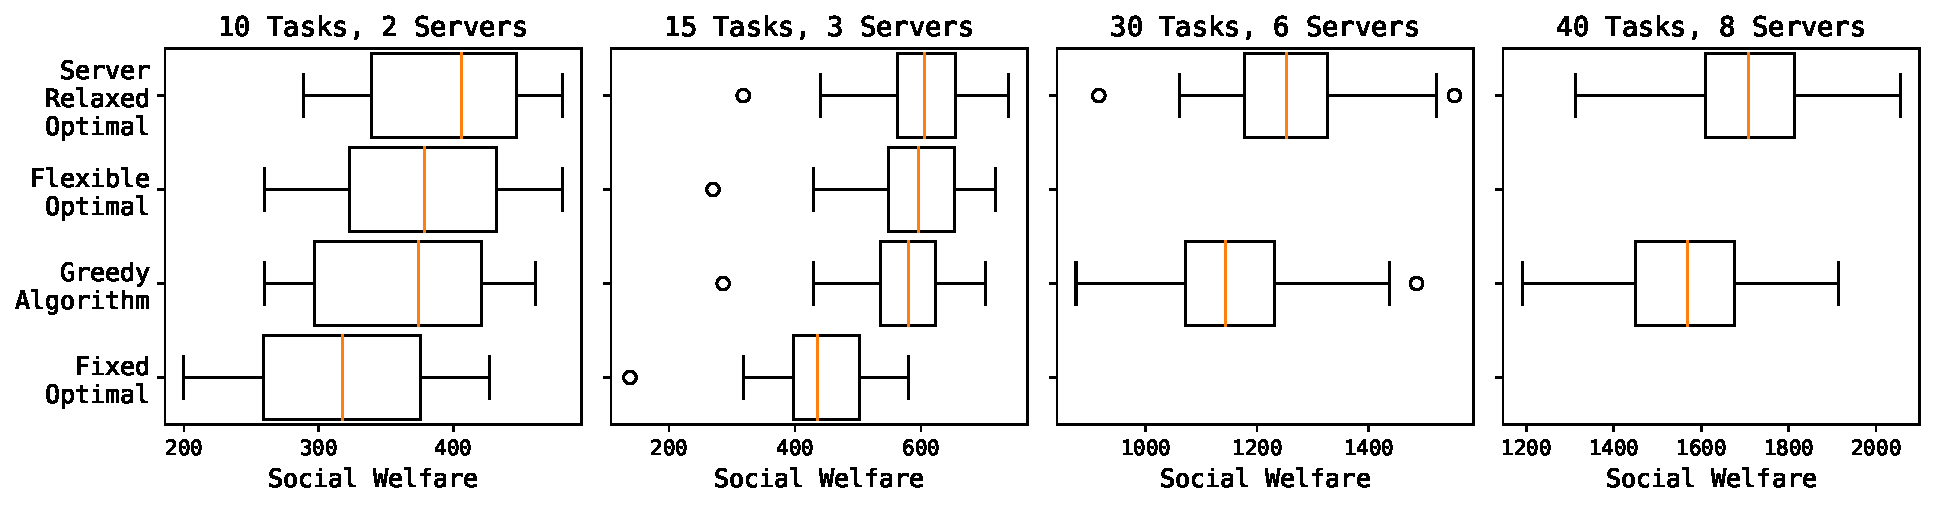
\includegraphics[width=\textwidth]{figs/greedy/social_welfare.pdf}
    \caption{Social welfare of the server relaxed optimal, flexible resource allocation, greedy algorithm and fixed resource allocation for a range of model settings.}
    \label{fig:greedy-algorithm-comparison}
\end{figure*}

\subsection{Properties of the proposed algorithms}
In this section, we have presented three mechanisms to solve the optimisation problem proposed in Subsection~\ref{subsec:optimisation-problem}. Table~\ref{tab:algorithms-properties} considers a range of important properties that allow an easy comparison between the proposed algorithms.

\label{subsec:proposed-algorithms-properties}
\begin{table}[H]
    \caption{Properties of the proposed algorithms: greedy algorithm, critical value auction and the
             decentralised iterative auction}
    \label{tab:algorithms-properties}
    \begin{tabular}{|p{2.25cm}|p{1.5cm}|p{1.25cm}|p{2cm}|}
        \hline
        \textbf{Properties} & Greedy algorithm & Critical value auction & Decentralised iterative auction \\ \hline
        Strategyproofness & No & Yes & No \\ \hline
        Optimality & No  & No & No \\ \hline
        Scalability & Yes & Yes & No \\ \hline
        Task information & All & All & All except the task value \\ \hline
        Decentralisation & No  & No  & Yes \\ \hline
    \end{tabular}
\end{table}